\documentclass[review]{elsarticle}
\usepackage{hyperref,lineno}
\usepackage{xcolor}
\usepackage[utf8]{inputenc}
\modulolinenumbers[5]


\newcommand{\memo}[2]{\textcolor{#1}{#2}}
\newcommand{\maria}[1]{\memo{red}{#1\\}}
\newcommand{\xavi}[1]{\memo{magenta}{XRC: #1\\}}

%\journal{Journal of Archaeological Science}


\bibliographystyle{model2-names.bst}\biboptions{authoryear}


\begin{document}

\begin{frontmatter}

\title{The markings of the trade: exploring the patterns of olive oil production in Roman Baetica}

\author[ceipacadress]{Maria Coto-Sarmiento\corref{mycorrespondingauthor}}
\cortext[mycorrespondingauthor]{Corresponding author}
\ead{mcotsar@gmail.com}


\author[edadress]{Xavier Rubio-Campillo}

\address[edadress]{School of History, Classic \& Archaeology, Room OOM.33, William Robertson Wing, Old Medical School, Teviot Place, University of Edinburgh, UK}
\address[ceipacadress]{CEIPAC, Department of Prehistory and Archaeology, Montalegre, 6-8, 08001, University of Barcelona, Barcelona, Spain}

\begin{keyword}
Roman Empire; amphora workshops; Dressel 20; social learning; cultural evolution
\end{keyword}



%cambiar quizás
\begin{abstract}

The aim of this study is to explore economics dynamics in the production and distribution of olive oil trade. 
Our case of study has been focused on the production processes located in Baetica province (currently Andalusia) from 1st to 3rd AD. In particular, we want to detect patterns of olive oil production that link amphora workshops and amphoric stamps. Baetica became important production and distribution centre during the Roman Empire. However, it remains under debate how this province was organised and whether it could be possible to identify patterns in the olive oil market. Amphoric stamps are used to identify the presence of different groups that might share similar stamps. To achieve this goal, we analyse a set of stamps from two centres: 1) producer centres by analysing different workshops in Baetica province and 2) two Roman provinces such as Germania and Britannia as a receptor centres. They will be used to detect a relation between the distribution of amphoric stamps and the economic structure in both centres. Here we use methods borrowed from Ecology that allow us to identify if amphora workshops share similar amphoric stamps depending on the spatial distance. 

The analysis explores how quantitative approach provides a useful tool for the interpretation of the economic processes. Finally, results pretend to highlight the organisation of Baetican olive oil production in the Roman Empire linked to the differences observed in the archaeological evidence.

\end{abstract}


\end{frontmatter}


\section{Introduction}


%primer párrafo más general---- especifico (¿dónde se ha aplicado?)
Material culture is one of the most frequent indicator of trade in the archaeological record. In archaeology, they allow us to highlight a part of mechanism of production and distribution of goods along the Mediterranean \citep{bevan_mediterranean_2014}. Particularly, the spread of these factors had an important impact during the Roman Age, when the progressive exploitation of communication networks allowed a major interaction between communities \citep{orengo_seeds_2016}. Given this fact, an important mechanism of production control under Roman government was created spreading by different areas attending to the richness of different places. Roman provinces such as Baetica (currently Andalusia, south Spain) became important production centres of olive oil during the Roman Empire. Olive oil was considered as the liquid gold since it was used in different aspect of the daily life as cooking, hygiene or lighting  \citep{mattingly_d.j._oil_1988}. As a consequence, this product was distributed in a large number of amphorae along the province, mostly to supply the Roman Army and Italy \citep{blazquez_exportacion_1980}. 


Despite this issue has been widely discussed over many decades, the understanding about the production processes is still under debate, mostly due to the lack of written records. The application of different quantitative approaches combined with the archaeological evidence has allowed us partly to deal with the complexity of understanding the Roman production \citep{orengo_seeds_2016,
brughmans_roman_2016,coto-sarmiento_identifying_2018,bayesian_2018}.


%This paper explore--- resumir en dos líneas el objeto de estudio y definir que ha sido usado para ello dispersion of culture
This paper aims to understand the production dynamics in connection with a different areas within Roman Empire. Specifically, our work pretends to detect microeconomic processes focused on a commercial product from a specific province \citep{isaksen_network_2006}. We want to detect the pattern of olive oil production that link amphora workshops and amphoric stamps used to mark them. We focus here on exploring the economic relation between stamps and amphora production and distribution centres. To do this, an Ecology approach has been used to analyse the dispersion of stamps between amphora workshops \citep{rubio-campillo_ecology_2018}. 

\maria{deberia cerrar esto}



\subsection{The Amphoric production in Baetica province}


The high demand of Roman provinces stimulated by the good condition of the Baetica lands allowed to develop a massive infrastructure of olive oil production. The production and distribution of olive oil were growing exponentially during almost three centuries \citep{remesal_concierto}. As a result, hundreds of amphora workshops were made to support this high demand of Roman Empire. These workshops were located along the rivers Guadalquivir and Genil, supplying from the riverine connectivity to the Mediterranean and Atlantic routes \citep{garcia_vargas_enrique_formal_2010}.

The majority of olive oil amphorae produced in this province and shipped through the provinces belong to Dressel 20 type \citep{dressel_ricerche_1878,
millet_anforas_1998}. This amphora is commonly associated with the transportation of Baetican olive oil during the Roman Empire \citep{berni_millet_epigrafianforica_2008}. Most Dressel 20 were marked in stamps, inked in \textit{tituli picti} and incise in \textit{graffiti} with different information still unknown. Indeed most of the inscriptions on the amphora have not enough analysed due to the fragmentation of the material or the shortage of samples \citep{aguilera_evolucion_2007,rovira_guardiola_grafitos_2007}. 


\subsection{A potential indicator of Roman economy: Dressel 20 stamps}

Stamps are the most studied in this type of amphorae. The fascination aroused by stamps has caused it to be one of the inscriptions with the most publications about its origin and meaning. Its endure in time become it an essential element that were used to mark amphorae during almost three centuries \citep{remesal_sellar_2016} (Fig.\ref{amphora}). 

\begin{figure}[htp]
	\centering
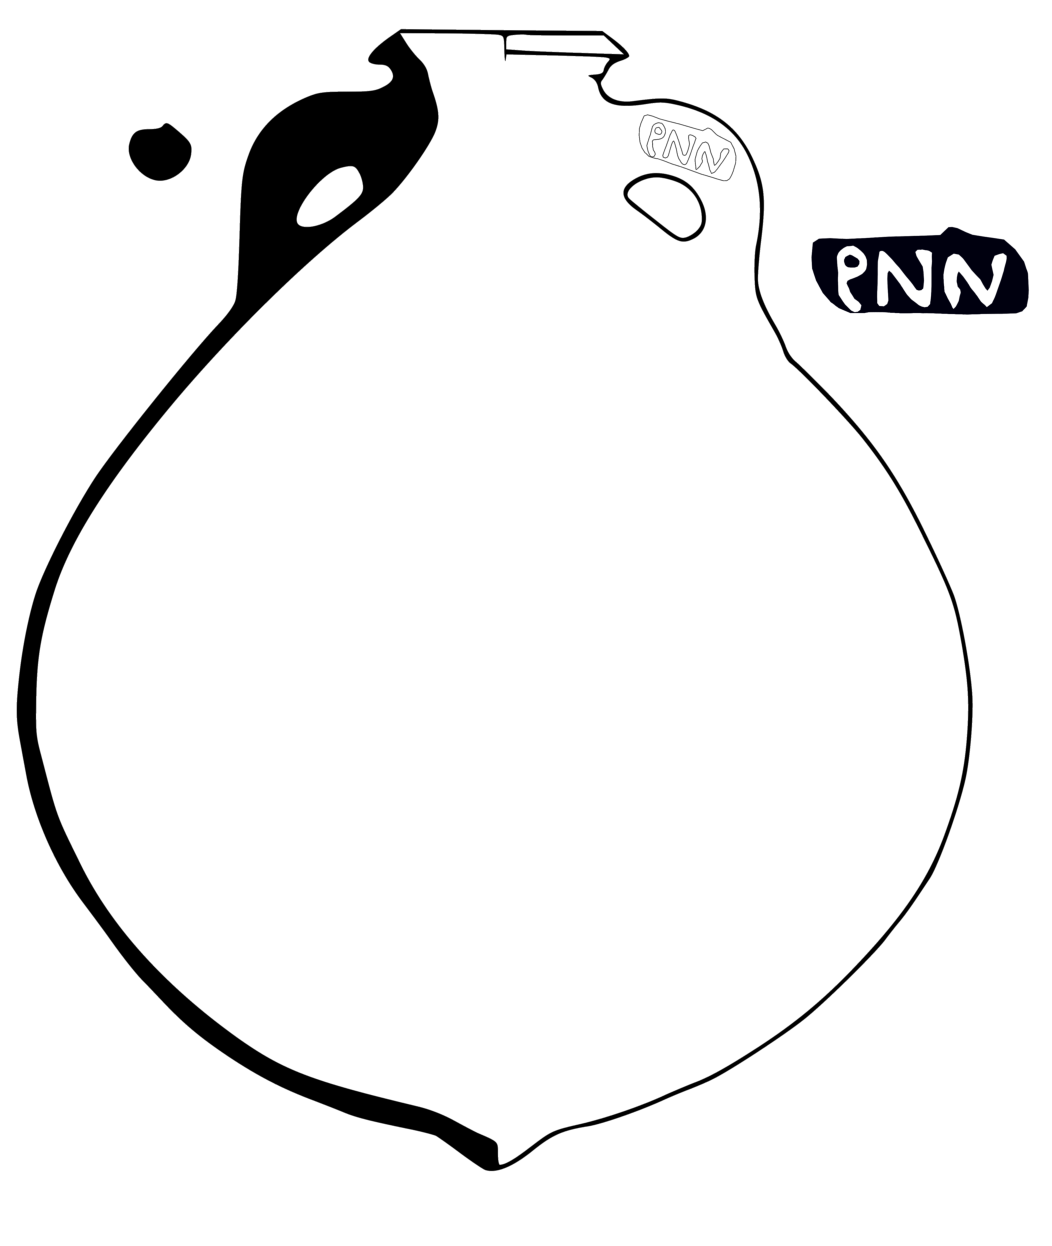
\includegraphics[scale=0.5]{figs/dressel20}
\caption{Dressel 20 were mostly marked with stamps of three letters called \textit{tria nomina}}
\label{amphora}
\end{figure} 

Frequently, they were marked mainly in handles but seldom in rims and body \citep{millet_anforas_1998}. 
The information of the stamps is shown in different forms and letter content and it seems that there was not a unique criterion. Stamps are mostly formed by a code of three letters and they can appear in a abbreviated form or complete and they are known as \textit{Tria Nomina} \citep{berni_millet_amphora_1996}. Despite researchers identify stamps as a identity marks, there is not a general consensus about the meaning of the stamps \citep{rodriguez_baetican_1998}. Alike most Dressel 20 containers were not stamped being difficult to determinate. 

They could be identified based on three premises: content (olive oil), context (amphora workshop) and subject (individuals involved). On the one hand, it seems that stamps could have been identified as the land owner of the olive groves \citep{rodriguez_economioleicola_1977}. On the other, they could belong to the owner of the making amphorae workshops or even a group of amphora workers \citep{berni_millet_epigrafianforica_2008}. In any case, the use of these stamps became in a good proxy to define somehow the system of working in the workshops. 

%Hyphotesis
Nevertheless, some challenges remain under discussion such as how this production was organized and whether it is possible to distinguish production patterns in the olive oil trade. Our questions will be focused on the distribution of amphoric stamps. Did they follow a distribution pattern? Did stamps share the same workshop? Neither written records have been found that it could explain the economic role of Baetica province in the Roman organization. Indeed, archaeological evidence shows a highly specialized production with a long activity in a this specific area with apparently few changes \citep{remesal_anforas_2004}. 

%hipotesis: si esto es así entonces es asá

The assumption of this study is analysing the effect of the production patterns between different centres. We are specially interested in identifying links between producers and consumption centres using amphoric stamps. To do that, we use the CEIPAC database to collect the stamps from different places. The CEIPAC dataset contains over 50.000 of epigraphy records found in amphorae, mostly from \textit{Monte Testaccio}.

Three case study have been studied in order to analyse the relation between production centres (Baetica) and consumption centres (Britannia and Germania). In the case of Baetica province, we want to identify the role of the stamps in the organisation of the workshop. In Roman provinces, our aim is detecting groups of stamps concentrated in a area or if some groups have an important role for the exportation of olive oil in those provinces. This economic connection could affect due to different aspects: a) correlation between spatial distance and centres based on the idea that closer workshops concentrate similar amphoric stamp in a specific area than the distant workshops and b) groups of similar stamps were concentrated in a specific Roman province. 

Therefore, this study proposes an evolutionary baseline to explore the distribution of Baetican olive oil production by computing spatial correlation between stamps. A way to analyse is by using a quantitative framework to measure the similarity. Here we use a ecological approach based on three steps: a) to detect similarities between stamp codes, b) to explore a potential spatial correlation and c)to establish a correlation between similarity of stamp and spatial distance. 






%this paper aims to highlight the production dynamic in connection with the proximity between amphora workshops and stamps. 


\section{Material and methods}

\subsection{Production centres: Baetica province}

Our case study examines the relation between the distribution of amphoric stamps and the workshops. In particular, we study the distribution of amphoric stamp with the aim of identifying a correlation between geographical distance and amphoric stamps. Based on this assumption, we proposed three hypotheses: a) it exists a correlation between spatial distance and the distribution of stamps, b) stamps located in close workshops share similar traits and c) Low mobility of amphoric stamps to other region: stamps always stay in the same region.  

The amphora workshops were situated in different locations in Baetica province, along the river Guadalquivir and its tributary Genil in order to detect similarities between stamps from workshops and spatial distance (see Fig.\ref{workshop}).

\begin{figure}[htp]
	\centering
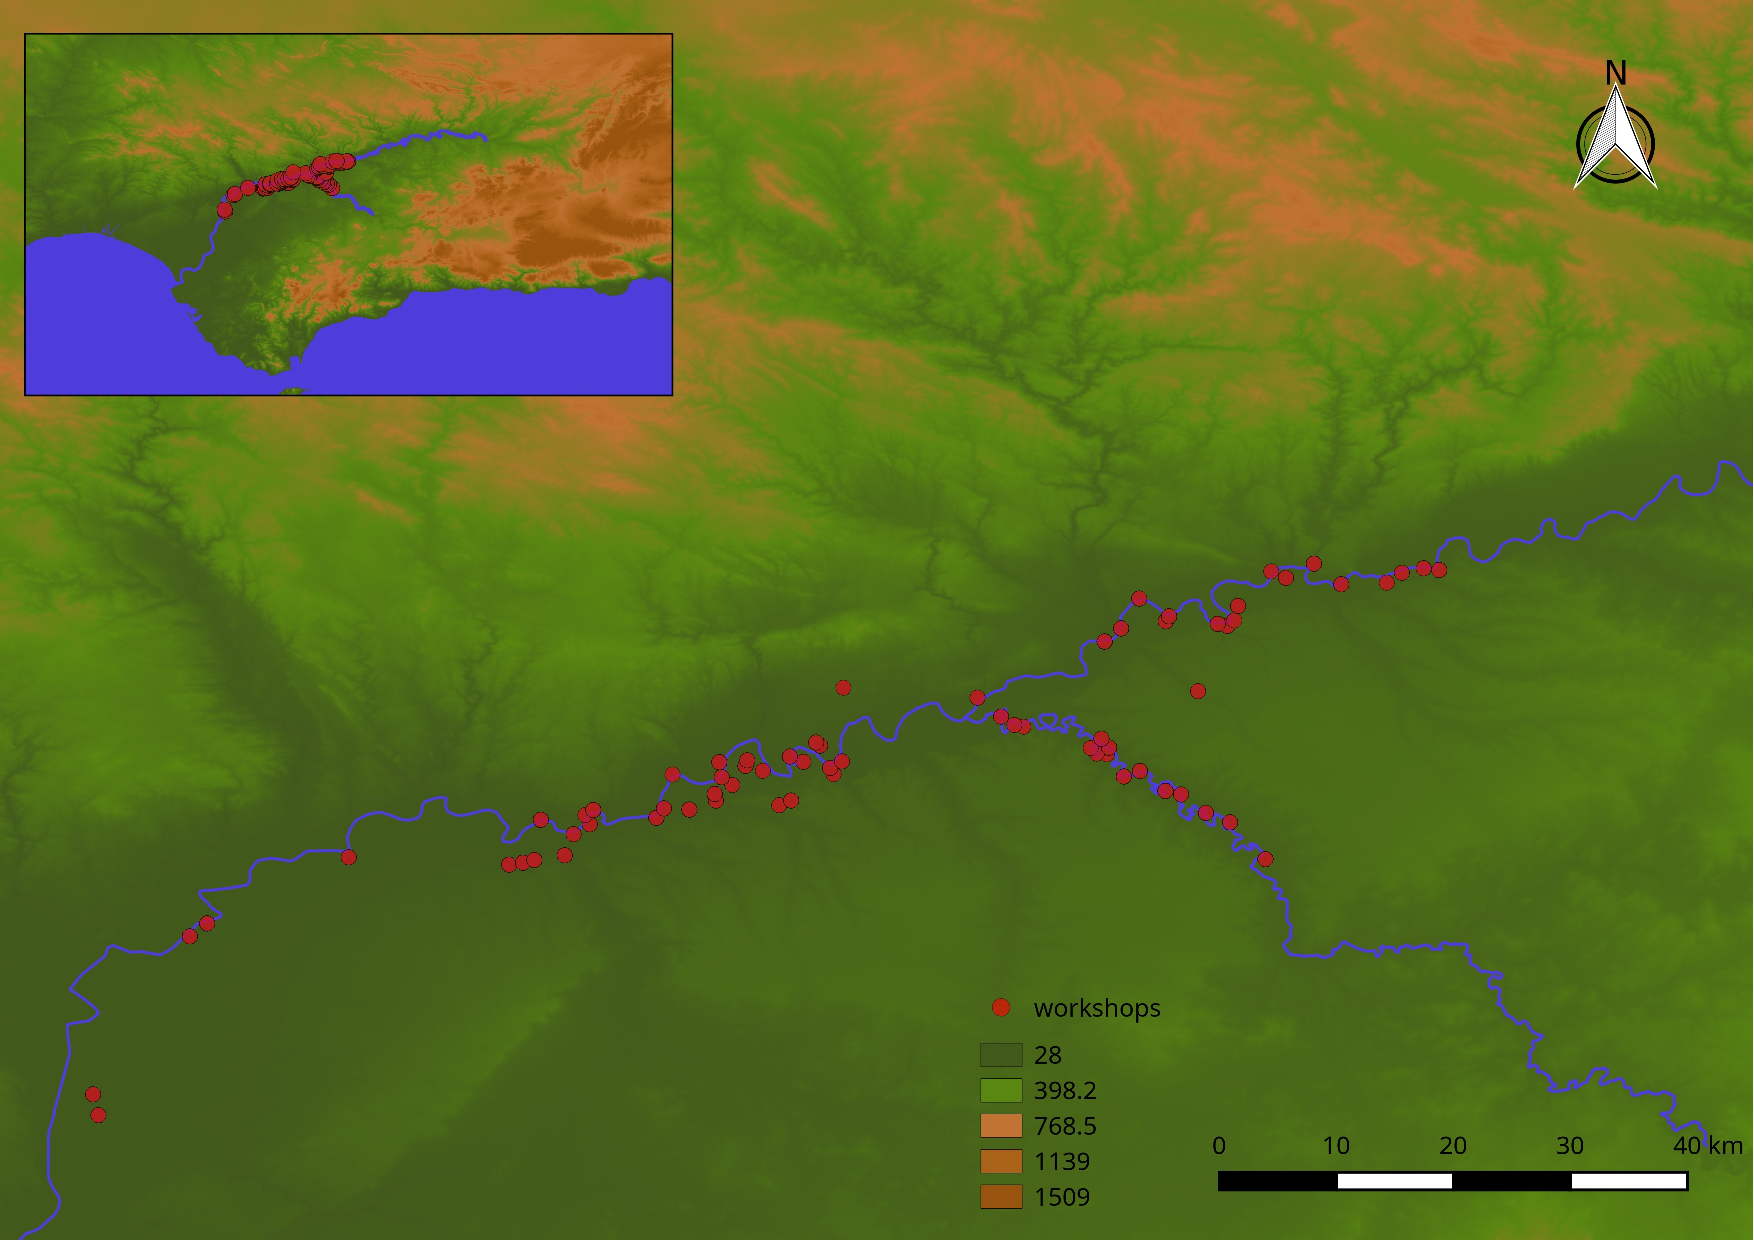
\includegraphics[width=\linewidth]{figs/workshop}
\caption{Distribution of the workshops}
\label{workshop}
\end{figure} 


The chronology in the workshops is widely diverse from the first to the third centuries AD \citep{millet_anforas_1998,rodriguez_baetican_1998,chic2005comercio}. Some stamps show a more specific chronology while the majority of them display a large activity of production that it can be difficult for specifying an accurate chronology. This could be due to two reasons; firstly, most of the workshops were partially excavated and focused on archaeological surveys in order to collect the maximum stamps as possible; secondly, Dressel 20 was produced during almost three centuries with apparently few changes \citep{berni_piero_chapter_2017}.

\subsubsection{Material}
 
We studied a dataset of 3798 stamps collected from different Dressel 20 amphora workshops in Baetica province. The stamp database was compiled by CEIPAC database \citep{remesal_centro_2015} (see CEIPAC database here \url{http://romanopendata.eu}). However, approximately the 70 \% of stamps cannot be tested due to fragmentation or incomplete information. Consequently, we discard integrate the fragmented stamps in our dataset. We finally filter a total sample of 987 stamps comprised of 130 different stamps from 81 workshops. 


%3798 = base de datos sin limpiar
%3791 = base de datos limpiada con cleanstamp.py
%3787 = no sé a qué corresponde pero es archivo baetica.csv

From the database, we collected the site where stamps were found and the stamp code. We also created a new column with the area of the stamps. These areas, known as \textit{conventus}, were administrative centres for territorial organization in the Roman Empire. Dressel 20 stamps were found in three different \textit{conventus}: \textit{Hispalensis} (currently Seville, hereafter Hispalis), \textit{Cordubensis} (currently C\'ordoba, hereafter Corduba) and \textit{Astigi} (currently Écija, Sevilla, hereafter Astigi) \citep{rodriguez_economioleicola_1977,
chicdatos2001,berni_millet_epigrafianforica_2008} .


\subsubsection{Exploratory Analysis}

We calculated the frequency of distribution in amphora stamps with the aims to carry out a exploratory analysis (EDA) to know the distribution and the number of stamps per each centre.  

The frequency of stamps per workshop can be seen in Fig. \ref{stamps}. Most stamps are distributed in only one workshop whereas few workshops concentrate a high frequency of different amphoric stamps. The type of distribution is also frequent in Roman economy where we observed a self-organized complex system patterns typical of a free market \citep{bayesian_2018}. 


\begin{figure}[htp]
	\centering
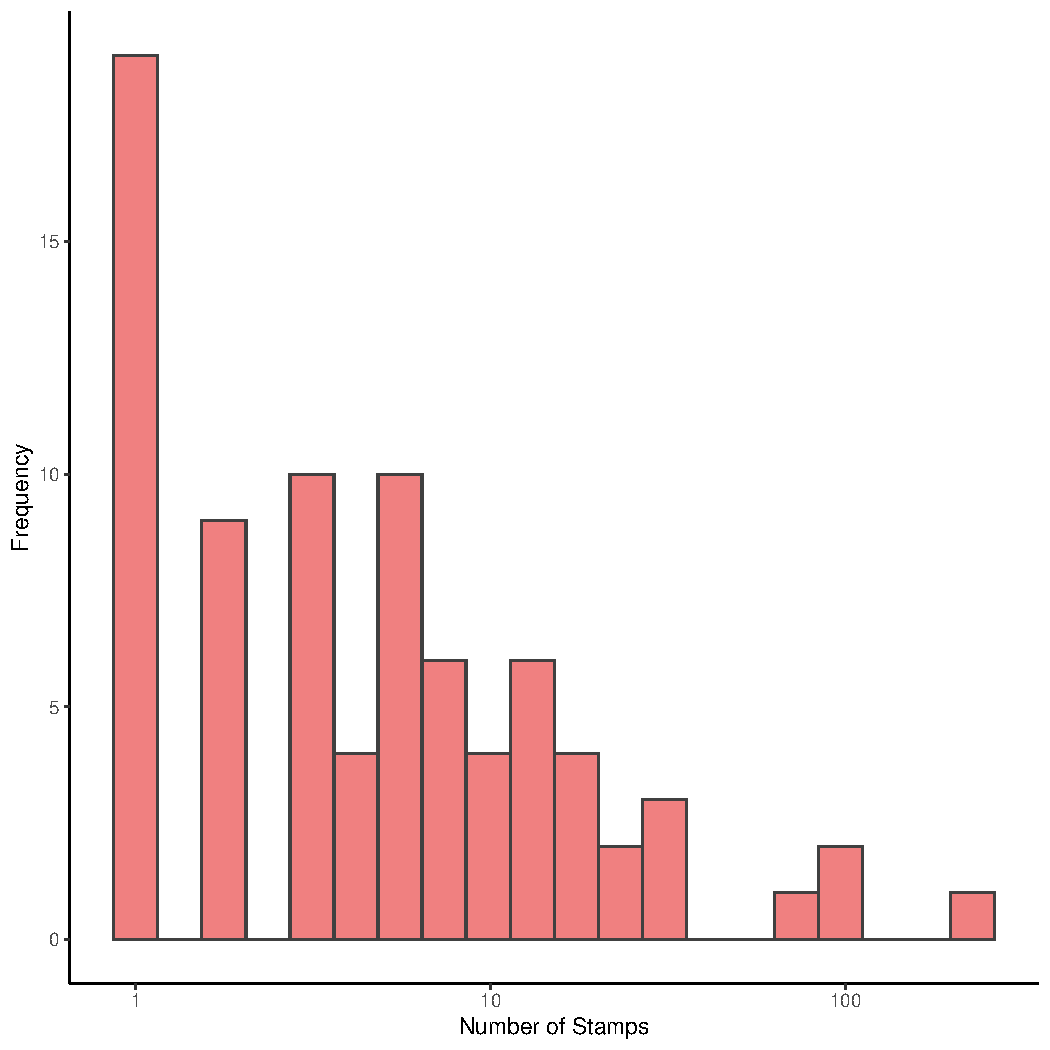
\includegraphics[width=\linewidth]{figs/frequencystamp.pdf}
\caption{Distribution of the number of stamps}
\label{stamps}
\end{figure} 


The distribution of amphora stamps in different \textit{conventus} can be seen in Fig. \ref{frequency}. The majority of stamps found are concentrated in \textit{Hispalis} with 574 stamps while \textit{Corduba} and \textit{Astigi} with 267 and 146 stamps, respectively. Mostly, workshops show a homogeneity on the frequency of stamps except both La Catria and Arva that show a big amount of stamps with 29 different stamps. According to previous studies, those workshops became in most important centres of amphora production although they could have been more intensely prospected then others. \citep{arva_1997}.
 
\begin{figure}[htp]
	\centering
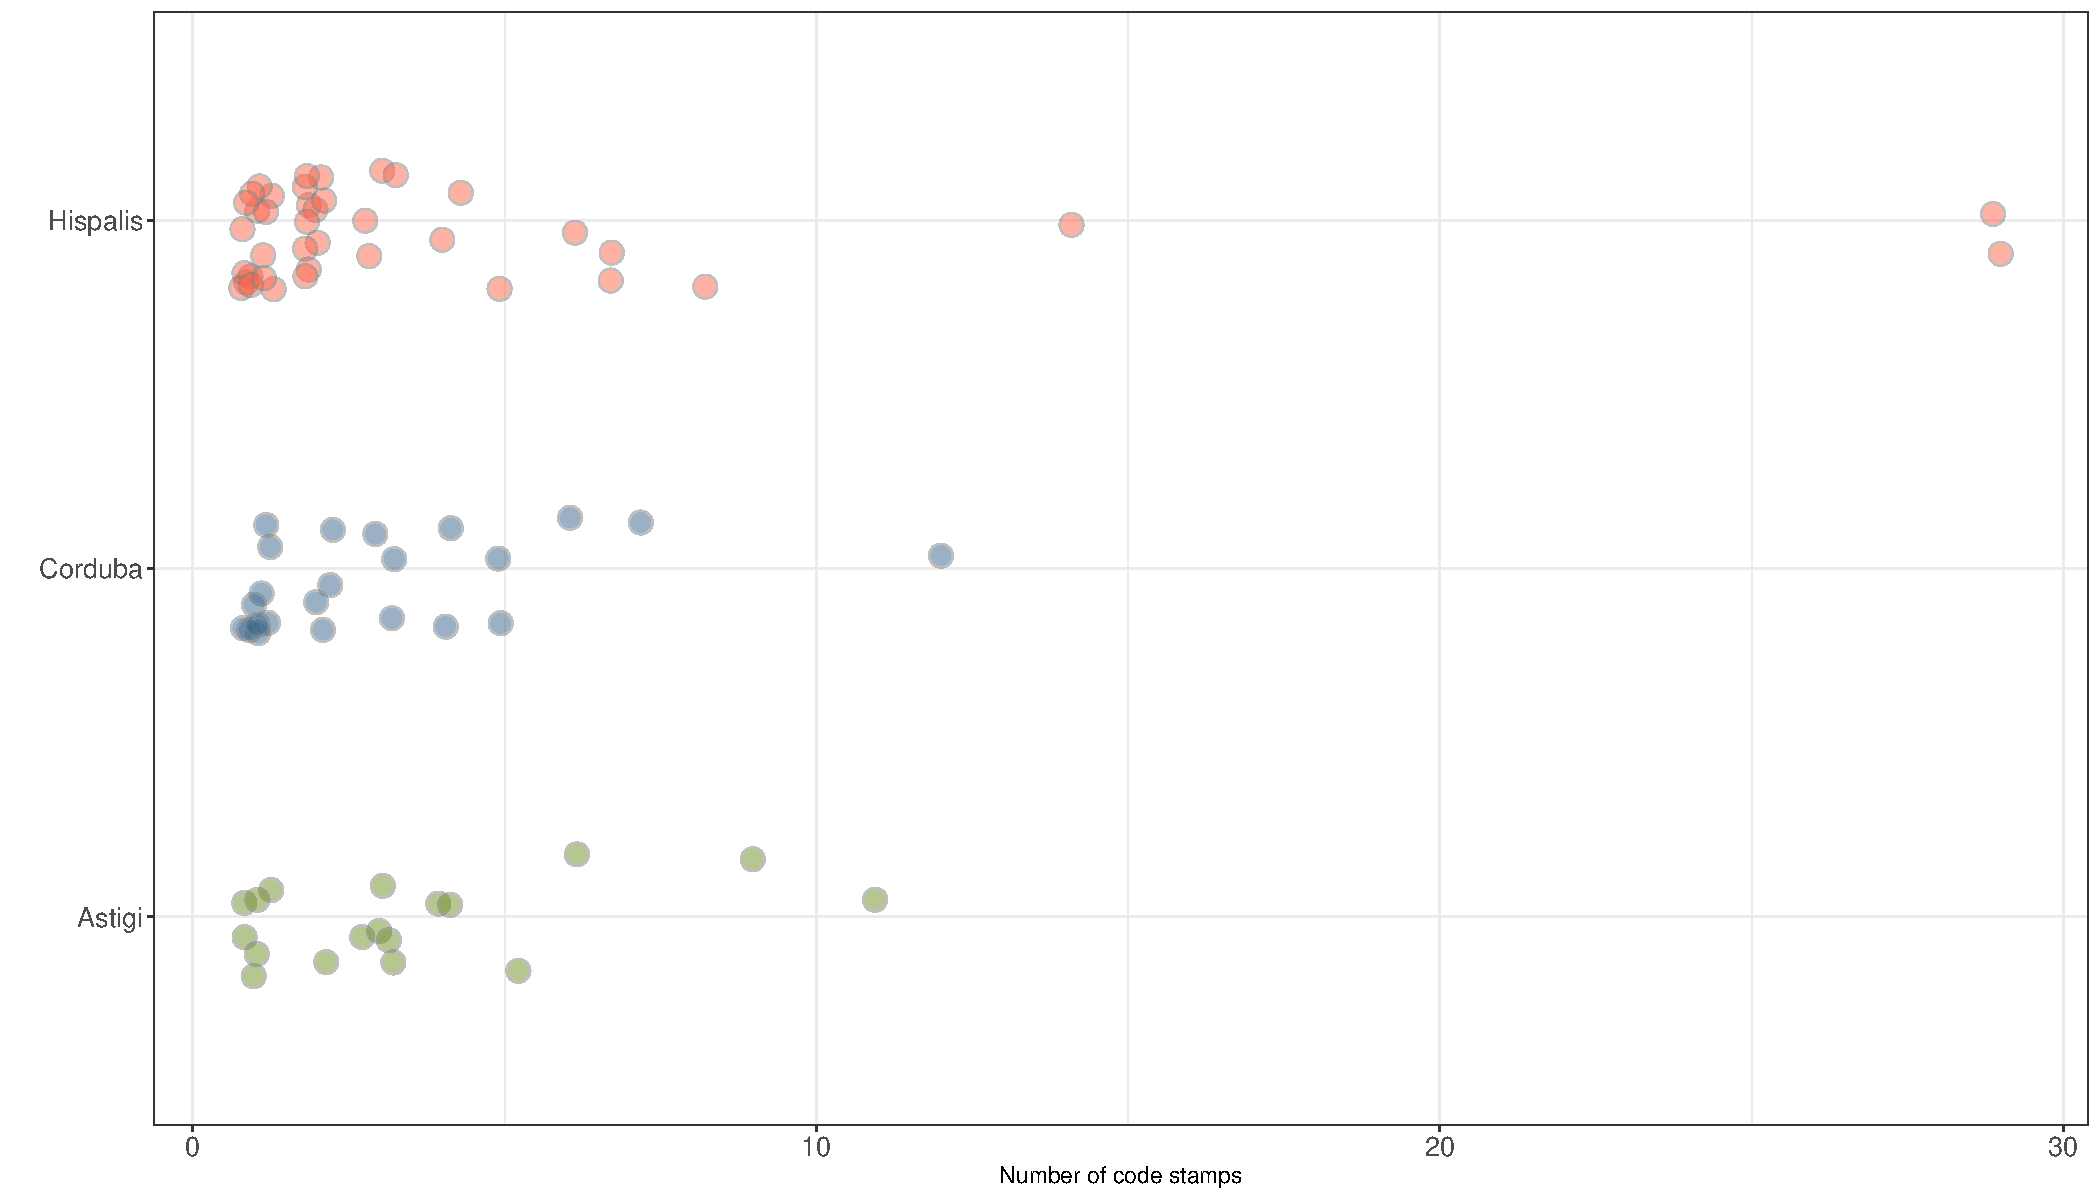
\includegraphics[width=\linewidth]{figs/frequency}
\caption{Distribution of the number of different code stamps for each area. Colors are represented by areas divided into Hispalis (red), Astigi (green) and Corduba (blue).}
\label{frequency}
\end{figure} 


\subsection{Consumption centres: Britannia and Germania}

The conquest of new provinces allowed to the Roman Empire the arrival of new resources. This lead to a progressive change in the economic and social structure. As a result, Augusto's administration created the figure of the \textit{praefectura annonae} for the supply of wheat. The role of the \textit{praefectura annonae} was mainly to provide though \textit{frumentationes} a quantity per month of wheat to Roman citizens \citep{remesal_annona_1986,remesal_concierto}. 

\subsubsection{Britannia}

The consumption of olive oil in Britannia was residual until starting the Roman conquest \citep{funari_corpus_1996,
carreras_abastecimiento_2003}.

It is well known that this product was not frequently consumed by autonomous population. The absence of olive oil importation before the conquest can be reflected by the shortage of this product until the arrival of high percentage of Dressel 20 amphorae to Britannia \citep[ 1]{carreras_britannia_1998}. Additionally, the land of Britannia showed inadequate for the olive oil production due to low environmental conditions. This issue was necessary for creating an important export apparatus from Baetica to supply Roman legions.
In this moment, we detect an increase of the olive oil exportation concurring with the displacement of Roman legions during the military campaigns \citep[161]{monfort_britanniaen_1998}. This fact will be spatial incidence in sites close at Hadrian Wall.  
Olive oil production in Baetica would cross the Atlantic until they reached the province and redistribute throughout the area from a series of strategic points \citep{carreras_atlantic_2012}. The increase of the exportation of Dressel 20 amphorae created an important commercial network for exchanges. Thus, the network was mainly focused on the support of soldiers during military campaigns. 
%debate intercambios puntuales o redes comerciales de abastecimiento

The presence of Dressel 20 stamps in military camps in Britannia have been widely studied in Roman archaeology \citep{carreras_britannia_1998}. This fact also indicates a possible governmental organisation allocate to reforce and supply of olive oil in military camps, such as Germania (Remesal Rodrıguez, 1986). However, it is unknown the type of economical system when managing or control the redistribution of olive oil in different sites in Britannia but it seems that it could have been in the main cities \citep[45]{funari_economic_2005}.

Finally, The increase in olive oil exports would experience a progressive slowdown
from the third century A.D., coinciding with the change in market strategy in the
Empire. In that moment, a progressive dicrease of Dressel 20 is documented being gradually replace for Dressel 23 amphorae. 


\subsubsection{Material}

We analysed a dataset of 2219 stamps from different centres in Britannia. 
%CITAR (Callender, 1965; Carreras Monfort y Funari,1998; Ayllón-Martı́ et al., 2018). 
The stamp database was also compiled by CEIPAC database. The database contained anomalies that were eliminated using the same criteria cited above. We finally selected the centres with more or equal than 5 stamps. As a result, we studied a total of 1765 stamps comprised of 968 different stamps from 46 centres.
The centres located in Britannia can be seen in Fig.\ref{britannia}.
 
\begin{figure}[htp]
	\centering
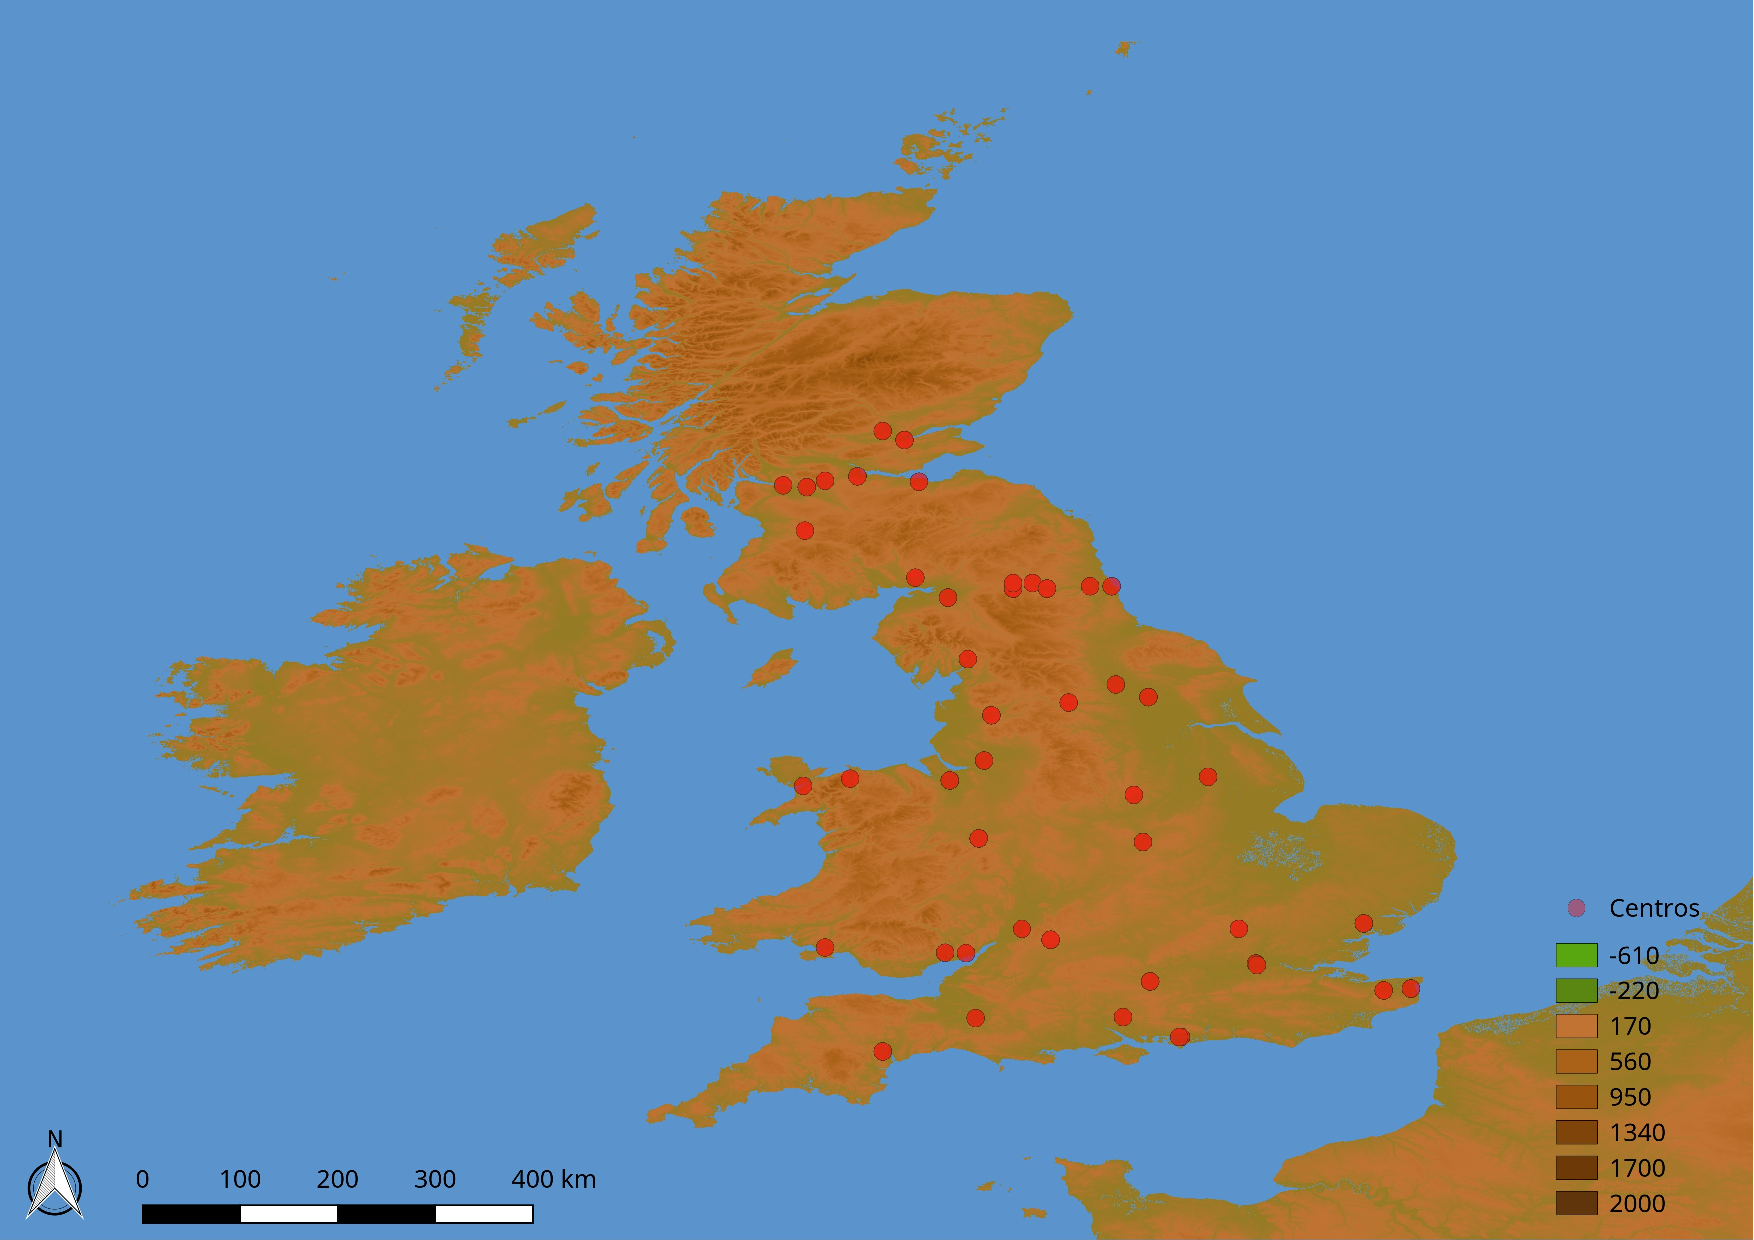
\includegraphics[width=\linewidth]{figs/britmap.pdf}
\caption{Distribution of centres in Britannia}
\label{britannia}
\end{figure} 


\subsubsection{Germania}

The Roman conquest in Germania dates from the end of the 1st century BC, during Caesar campaign and subsequently continued by Augusto. The advance of the Roman legions toward Gallia opened a way though the Atlantic Ocean to Germania \citep{remesal_annona_1986,
remesal_baetica_2002}.

It is thought that this route would have been initiated previously through 
terrestrial transport, although recent studies question this position giving an important role to the Atlantic route for both the conquests of Germania and those of Britannia \citep{remesal_germn_2010,rubio-campillo_ecology_2018}.

As the case of Britain, the consumption of olive oil in Germania was not detected before the conquest. 

The need to supply roman legions created a logistic network to supply to the army. In this moment, we detect the arrival of olive oil amphorae to Germania evidenced by the presence of Dressel 20 amphora in different sites close to limes. 

The roman studies about the presence of Dressel 20 amphorae has not been the same repercusion than the rest of the province. This can be explained due to the lack of data \citep{horacio2010llegada}.  

As a consequence, we do not the role that commerce agents in the participation of the distribution and exportation of olive oil in Germania or, on the contrary, the Roman army was the responsible to supply the product in the own province \citep[156]{remesal_germn_2010}. 


The presence of Roman army encouraged the exchange in the province showed by the arrival of this product both civil settlement and military sites with a mayor concentration at german limes. It seems that some baetican centres would be assigned to the support of olive oil. However, this hypothesis can not be proven by the lack of archaeological sources \citep[125]{remesal_concierto}. 


\subsubsection{Material}

We analysed a dataset of 2052 stamps placed in Germania. All the data was also compiled by CEIPAC database. We finally selected a total of 1621 stamps consist of 850 different stamps from 46 sites (see Fig. \ref{germania}). As previously before, the centres were selected with more or equal than 5 stamps. 


\begin{figure}[htp]
	\centering
\includegraphics[width=\linewidth]{figs/germania5.pdf}
\caption{Distribution of the sites in Germania. Most sites were located in limes during the Roman Empire}
\label{germania}
\end{figure}


%\subsubsection{Jaccard distance}
%The dataset was analysed using a statistic method as Jaccard distance. This method allows to measure the dissimilarity by calculating the presence of sets (CITAR). In our case, Jaccard distance was used to compute the mutual presence of traits in the amphora stamps but it does not consider the number of absences. A comparison was done with the distance of the workshops to identify whether there was an association between stamps and spatial distance amongst workshops. 


\subsection{Measuring the dissimilarity in stamps}


%quizás habría que hablar también del filtrado de códigos que se hizo en python porque antes había 3783 stamps pero se filtró por el número de letras...
%\xavi{lo del filtrado lo puedes poner de supplementary information con referencia al antiquity}

The approach proposed here is based on the idea of measuring the similarity between amphora workshops by quantifying similar stamps. A measure of dissimilarity has been chosen to analyse the dataset. We use the statistical technique Morisita-Horn index \citep{morisita_measuring_1959, horn_measurement_1966}. This method was performed to measure the dissimilarity between different samples of sets. Generally, it describes the dissimilarity between the system of two communities based on the idea of inverse correlation between diversity and species \citep{magurran_why_1988}.

The formula can be described as follows \citep{magurran_measuring_2013}:

\begin{equation}
D(MH) = 1- \frac{2 \sum(a_{i} \cdot b_{i})}{(d_{a} + d_{b}) \cdot (N_{a} \cdot N_{b})}
\end{equation} \\

$d_{a}$ and $d_{b}$ are given by the following equation:

\begin{equation}
d_{a} = \frac{\sum a_{i}^{2}}{N_{a}^{2}} 
\end{equation} \\

where $N_{a}$ is the total number of stamps in workshop A; $N_{b}$ is the total number of stamps in workshop B; $a_{i}$ is the number of different stamps for workshop A and $b_{i}$ is the number of different stamps for workshop B.

Considering our dataset as a non-uniform sample, this method provides a useful tool to handle large samples with different sizes and diversity \citep{wolda_similarity_1981}. Morisita-Horn index can be expressed considering 0 as total presence of similarity of stamps and 1 a totally dissimilarity between stamps. In our case, it will be calculated the number of times that one stamp appears in an amphora workshop. This method allows to bear in mind the similar number of times for each repeated stamp per workshop. If two workshops have similar stamp codes then the probability would be 0 whereas stamps codes are totally different when the results would be 1. 

%hablar sobre Horn (Morisita)hablar sobre que el sample no estaba uniforme por eso usamos el morisita horn

\section{Results}

\subsection{Production centres: Baetica Province}

The analysis shows that amphoric stamps could be correlated with the spatial distance. The correlation coefficients range from a minimum to a maximum. The dendrogram shown in Fig. \ref{dendro} was obtained with Morisita-Horn index. The dendrogram suggests that amphora workshops used different stamps for their production system. Nearby workshops show a similarity on the stamps while most of them seem to display different stamps roles. Additionally, groups of workshops sharing similar stamps were not found in the cluster: the majority of stamp grouping was composed by no more than three workshops. Indeed workshops that shared more similar amphoric stamps belonged to the same \textit{conventus} area, such as Picachos, Cerro de los Pesebres and El Castillejo. 

\begin{figure}[htp]
	\centering
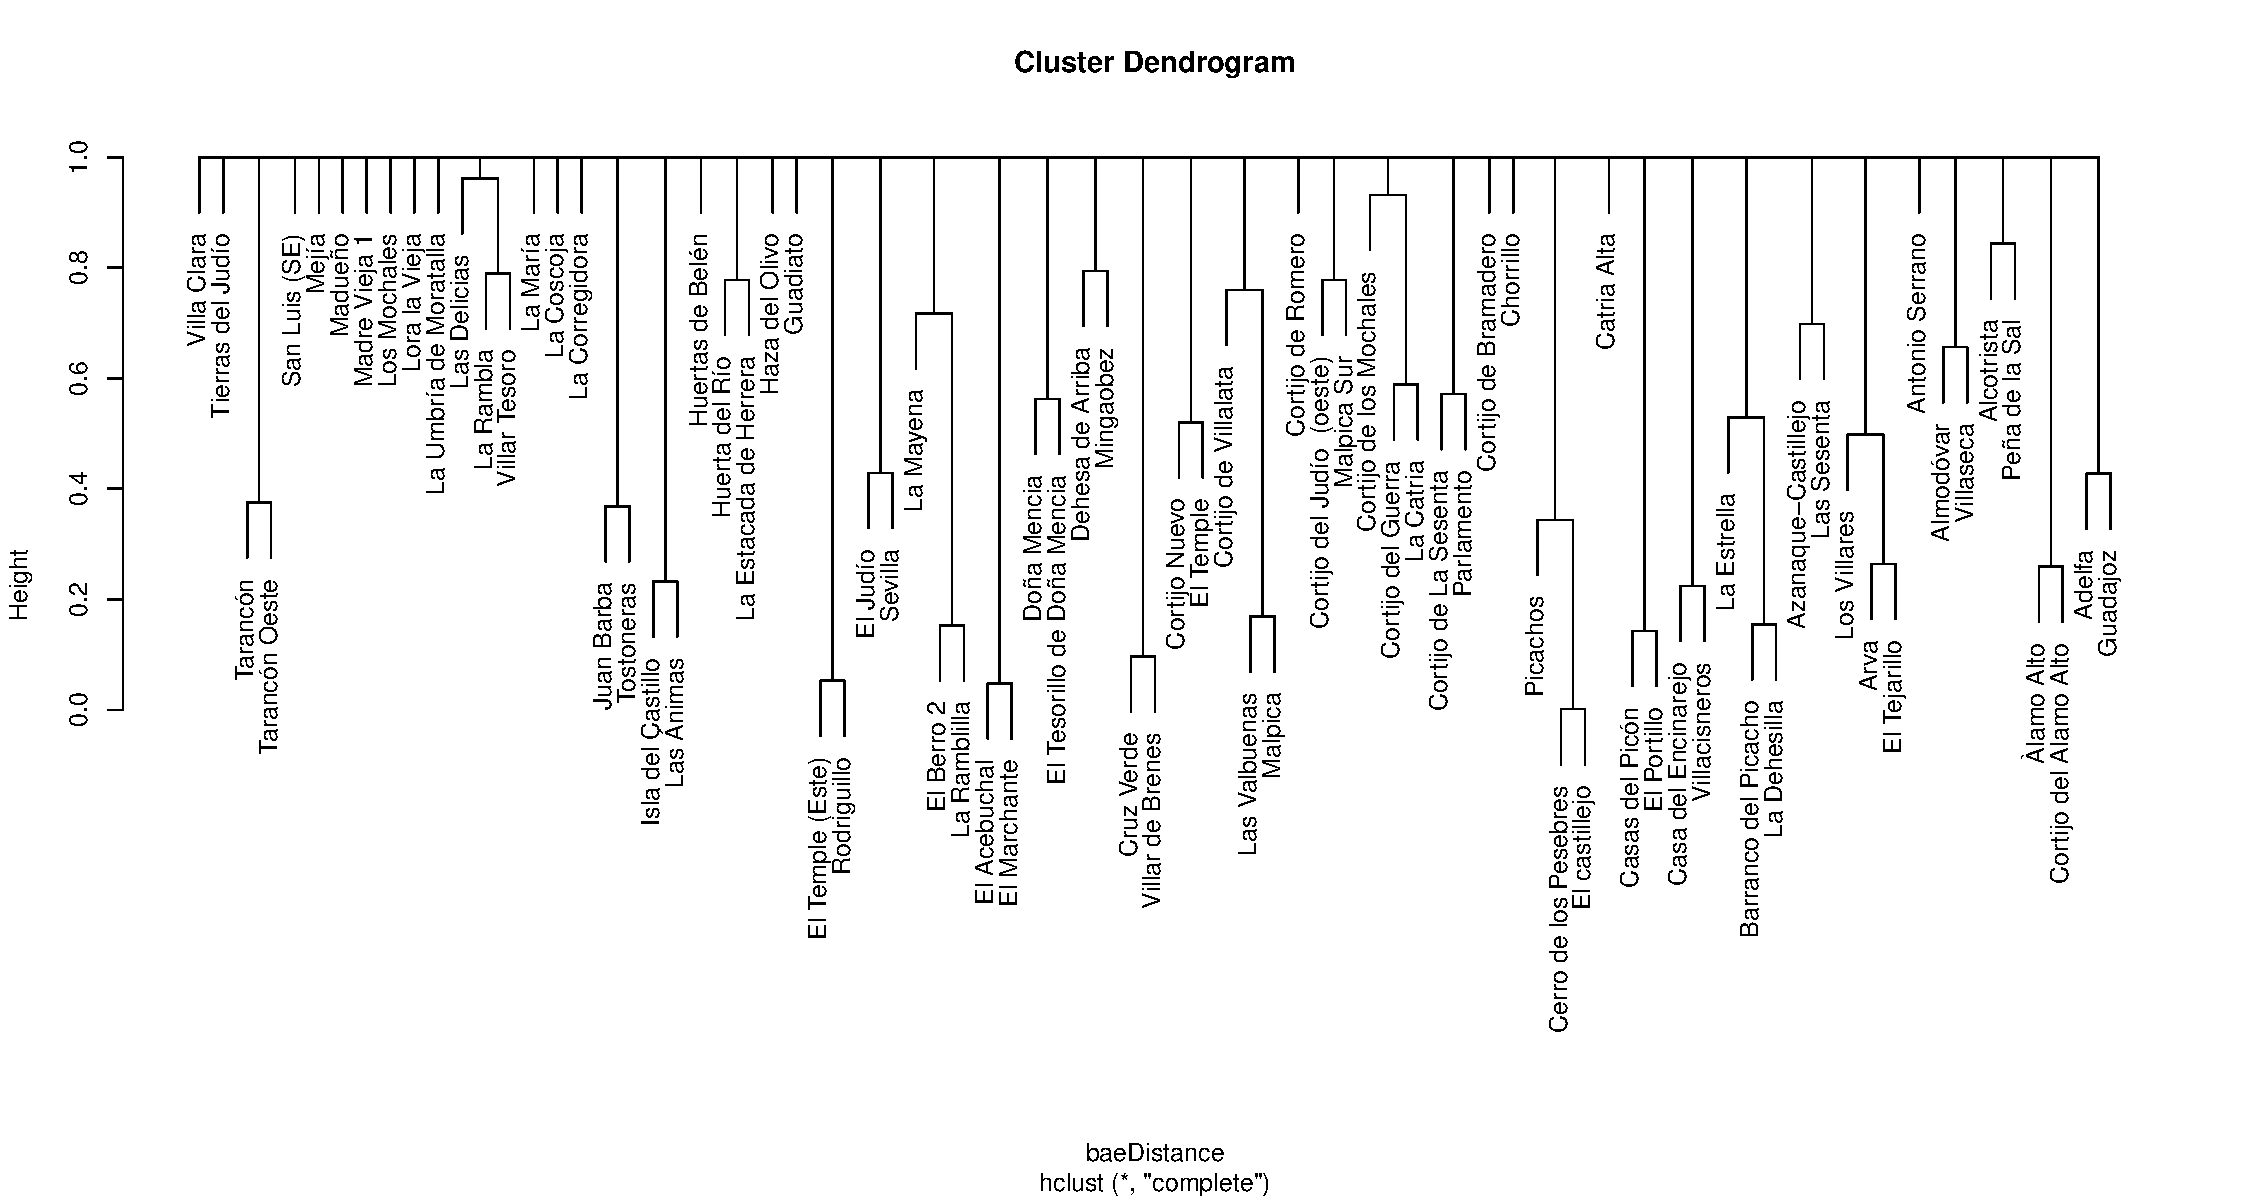
\includegraphics[width=\linewidth]{figs/dendro}
\caption{Dendrogram obtained by Morisita-Horn algorithm of different amphora workshops in Baetica area. Colours are represented by areas divided into Hispalis (red), Astigi (green) and Corduba (blue)}
\label{dendro}
\end{figure} 

\subsection{Reception centres: Britannia and Germania}

\subsubsection{Britannia}

The results show a correlation similar to the obtained in Baetica province. However, the similarity is less pronounced as we observed in the dendrogram in Fig. \ref{britmap}


\begin{figure}[htp]
	\centering
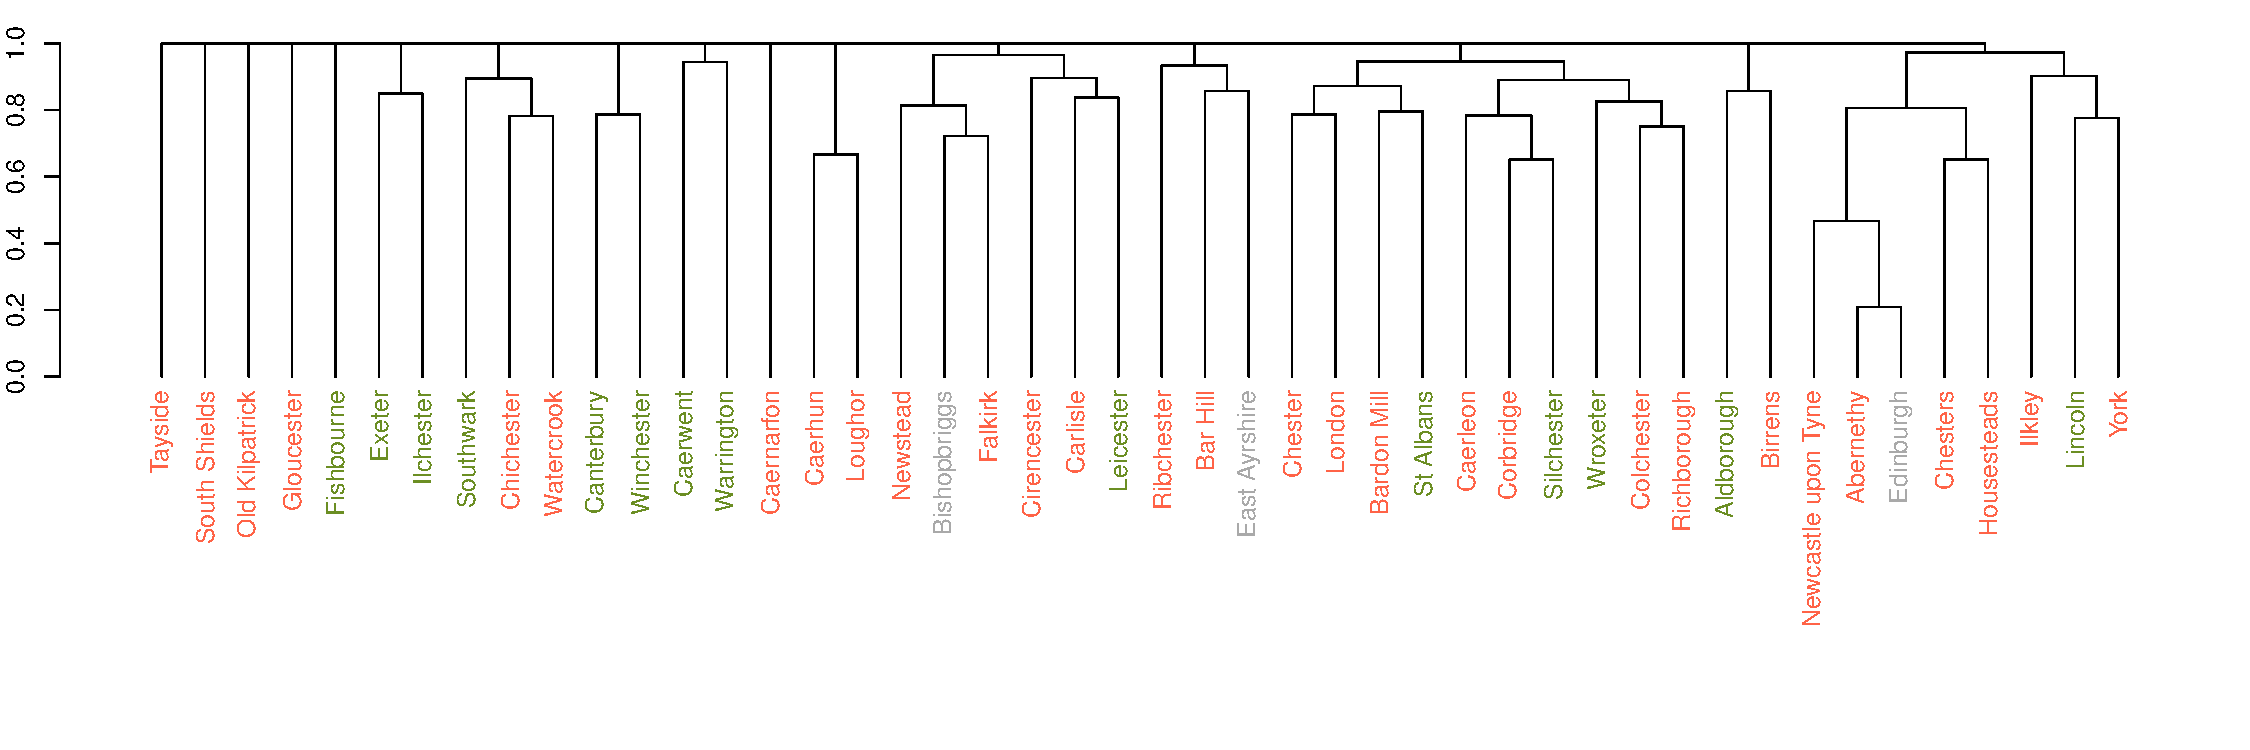
\includegraphics[width=\linewidth]{figs/dendrobrit5.pdf}
\caption{Dendrogram obtained by Morisita-Horn algorthm of different sites in Britannia. Colours are represented by type of sites divided into military sites (red), civil sites (green) and no specific (grey)}
\label{britmap}
\end{figure}


A minor correlation can be explained by the fact that Britannia spatial area is much wide than \textit{Baetica} where the centres were more concentrated.

Most military sites that showed greater similarity in the results were geographically close. We identified two factors in the results: 1) nearby sites tend to share similar stamps and 2) most sites have different stamps. 
By contrast, most sites did not show a strong similarity in stamp correlation. Neither we found a grouping of similar stamps in a specific place. In general, we did not observe any production pattern that indicates a clear organisation between production centres and reception centres. In other words, our results did not indicate the presence of a specific production center from Baetica in Britannia province. Rather it seems that olive oil production was distributed by non specific production centres. 


\subsection{Germania}

The similarity of stamps shows a results less significant than Britannia province as it can be seen in the dendrogram (Fig. \ref{germap}). 

\begin{figure}[htp]
	\centering
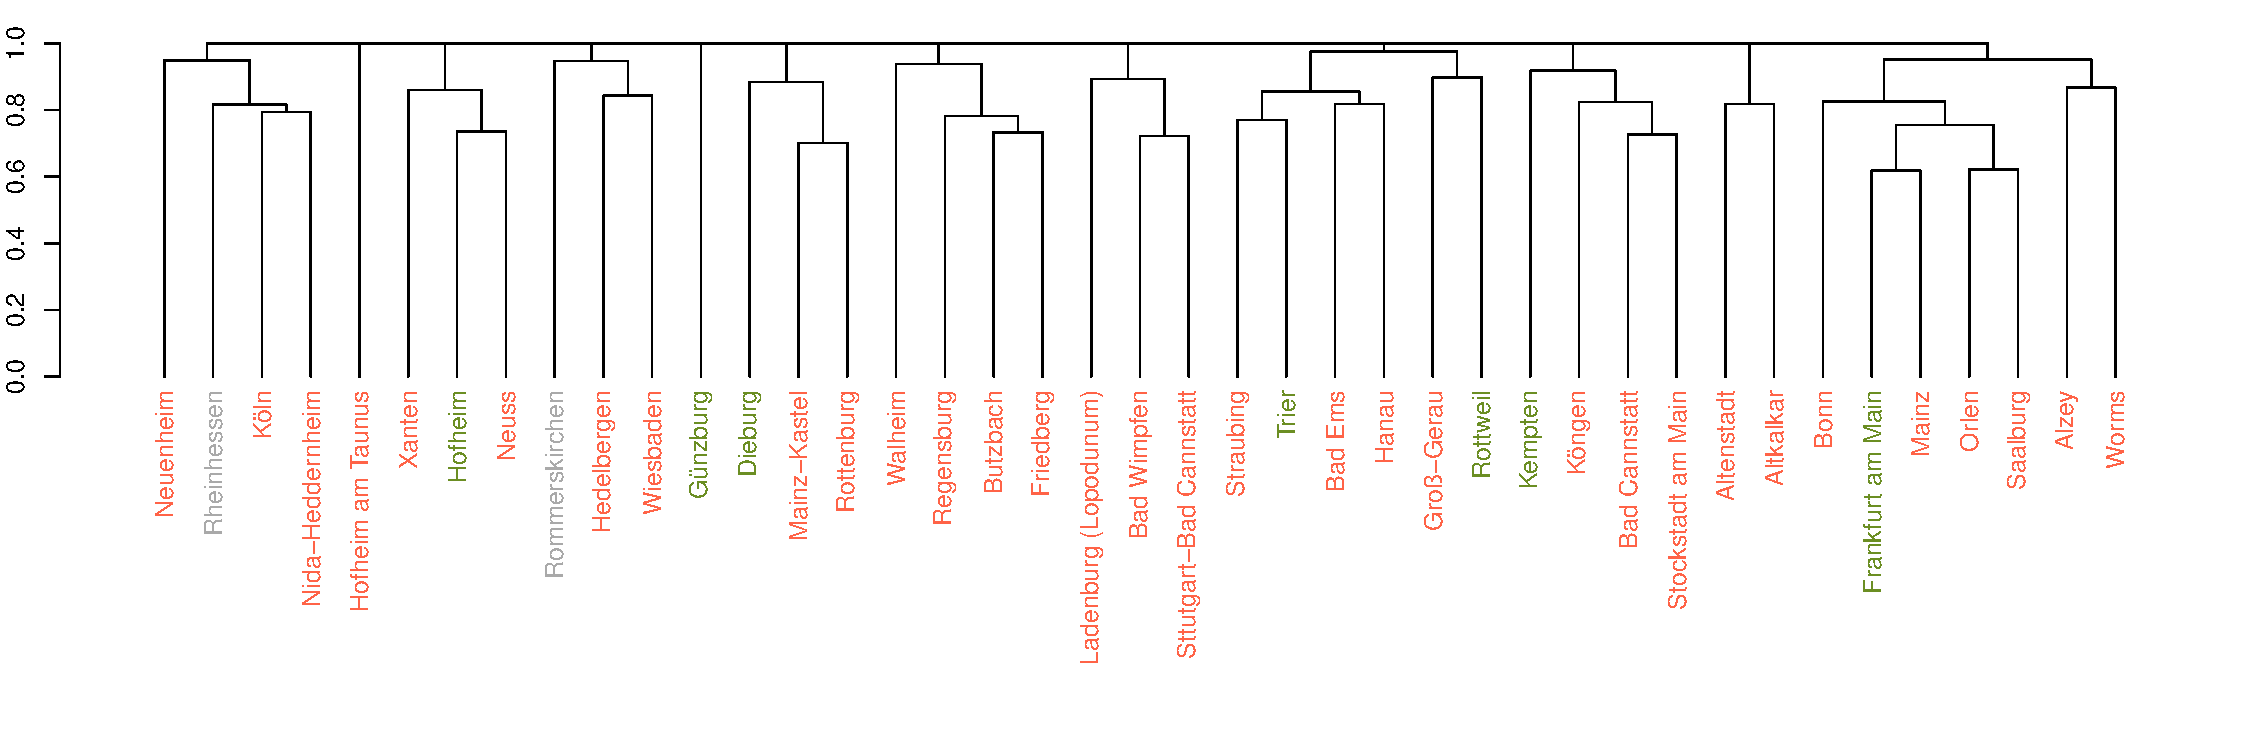
\includegraphics[width=\linewidth]{figs/dendroger5.pdf}
\caption{Dendrogram obtained by Morisita-Horn algorithm of different sites in Germania. Colours are represented by types of sites divided into military sites (red), civil sites (green) and no specific (grey)}
\label{germap}
\end{figure}


The sites with more similarity in stamps were closely located in limes. In this case, most sites have different stamps  which means that we did not detect any pattern. On the other hand, there seems to be a greater concentration of the seals in areas eminently militarised and close to the German limes. However, It is still no possible to determine with the data that the existence of a defined pattern that reflects in more detail the route of this production in the area of the German limes.


\section{Discussion and Conclusion}

%crear como una introducción

In this work, we aimed to analyse whether amphoric stamps could play an important role in the organization of the workshops along rivers. For this reason, dissimilarity index was used to detect differences among workshops and stamps. 

In our analysis, no strong relation between stamps and spatial distance have been detected in amphora workshops. The analysis suggests that there is not connection between stamps and the same amphora workshops, excluding certain exceptions when nearby workshops share the same amphoric stamp. Consequently, the majority of stamps are located in different amphora workshops and only similar stamps between closer amphora workshops were found. In any case, our results show that most similar stamps were detected in the same \textit{conventus} area. These stamps tend to share the same area of production but there is not a general relation between groups of amphora workshops and area. 

The hypothesis about groups of amphora workshops sharing the same stamps seems do not match with the results of the analysis even though there are similar stamps in closer workshops. Rather, it seems that each workshop were organized independently with different stamps. Those stamps detected in closer workshops do not move from other distant workshops. In other words, the stamps tend to keep in the same area and different stamps were located in a same amphora workshops. 

This could be defined by several factors. First, each workshop had a different organization involved to the use of stamps and they were not used in other workshops. Second, stamp similarity in closer workshops could be linked to a spatial pattern. It is more probably than closer workshops tend to share more traits than distant workshops. While the role of river was significant for the distribution of amphorae in consumption places, river connection amongst workshops does not seem show a relevancy for the distribution of stamps. Finally, the distribution of stamps could have shown some research bias. In some cases, workshops have been catalogued with different names in spite of belonging to the same workshops or being closer between each other. Additionally, most of the workshops were not widely excavated. 


The results of the case study could be interpreted by several reasons. On the one hand, the use of these amphoric stamps could have been exclusively running by the owner or owners of the workshop to distinguish the amphora workshop. This hypothesis would explain the fact that we do not find similar stamps in different workshops; however, we found different amphora stamps in the same workshops that they would be barely difficult to assign different owners. On the other hand, it could be interpreted somehow a batch systematic organisation. Considering that Dressel 20 was not marked in most cases, some authors point out that potters marked amphorae to prepare and distribute the commodity to be shipped \citep{berni_millet_epigrafianforica_2008}. This method would be used as an identifier to count the number of amphorae of a branch \citep{juanmorostesis}. This method could also have served to identify different groups of potter workers working in the same amphora workshop. Potters could have marked the amphorae to distinguish different groups working in parallel \citep{li_crossbows_2014}. This it would explain wherefore why we detect different stamps in a same workshop. 
In any case, we do not have enough archaeological evidence that can validate the interpretations presented here and our results are certainly valid only with the context of our case study. 

As summary, this method presented here provides a potential tool to understand mechanisms of production based on the similarity of artefacts. This method have identified differences in the case of the amphoric production within Roman Empire. Accordingly, the results have highlighted for the interpretation of the complex economic processes connected with the archaeological evidence. 


%Dressel 20 marked in the 30-40\%

\section{Acknowledgements}
%completar 
The research was funded by European Research Council Advanced Grant EPNet (340828). We are grateful to Simon Carrignon, Juan Moros and Ignacio Morer for their useful suggestions.  
All data has been analysed and conducted in R program version 3.2.4, using the packages \textit{vegan} \citep{oksanen_vegan_2007}, \textit{ggplot2} \citep{ggplot2:_2016}. Source and code are available at \maria{incluir github}. 


\section{References}

%\bibliography{bibliotex}
\bibliography{bibtesis}



\end{document}
